\section{Synteny}

\subsection{Methods}

\subsubsection{Macrosynteny}
\textcolor{red}{pipeline}

\subsubsection{Microsynteny}
\textcolor{red}{Synchro}

\subsection{Results}

\subsubsection{Genome Assembly Analysis}

\begin{figure}[H]
  \centering
  \begin{subfigure}[b]{0.45\textwidth}
    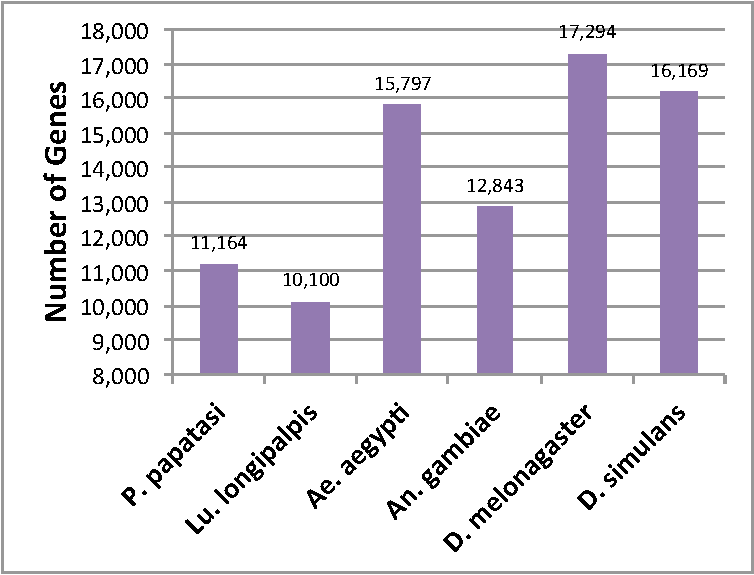
\includegraphics[width=\textwidth]{figures/synteny/genome_size_genes.pdf}
    \caption{Genome Sizes (Genes)}
  \end{subfigure}
  ~
  \begin{subfigure}[b]{0.45\textwidth}
    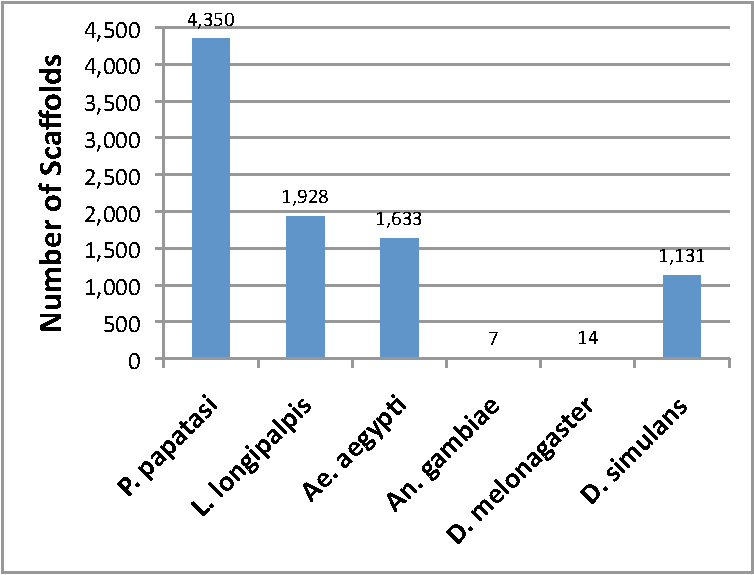
\includegraphics[width=\textwidth]{figures/synteny/scaffold_counts.pdf}
    \caption{Number of Scaffolds}
  \end{subfigure}
  ~
  \begin{subfigure}[b]{0.45\textwidth}
    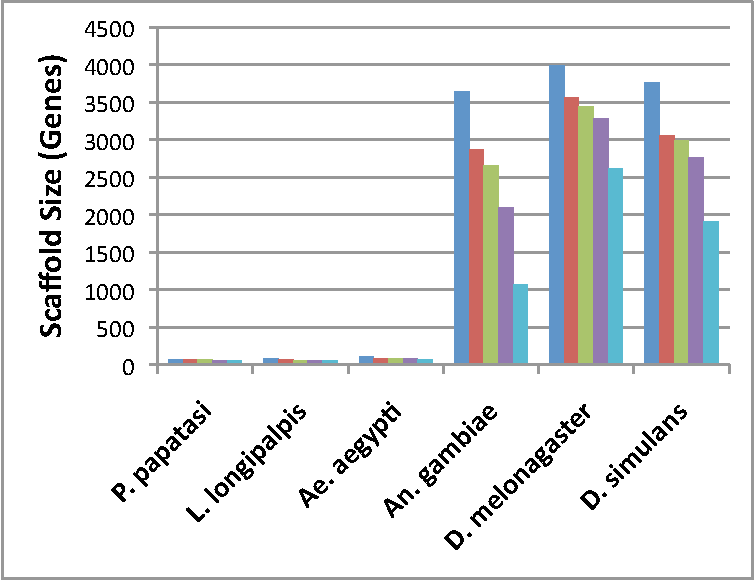
\includegraphics[width=\textwidth]{figures/synteny/top5_scaffold_sizes.pdf}
    \caption{Top 5 Scaffold Sizes (Genes)}
  \end{subfigure}
\label{fig:scaffolds}
  ~
  \begin{subfigure}[b]{0.45\textwidth}
    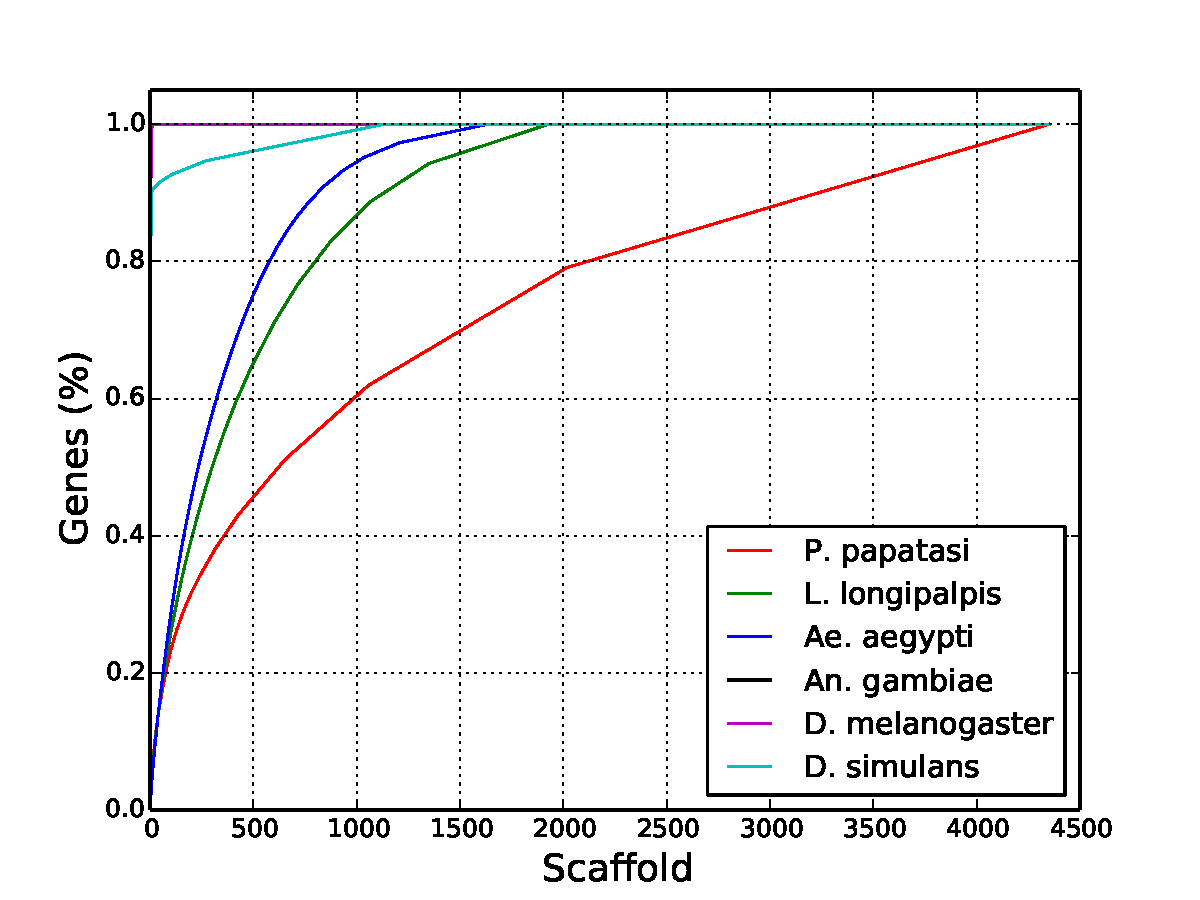
\includegraphics[width=\textwidth]{figures/synteny/gene_scaffold_cdf.pdf}
    \caption{Scaffold Genes CDF}
  \end{subfigure}
\end{figure}

\subsubsection{Phylogeny Tree}

\subsubsection{Macrosynteny}

\begin{table}[H]
  \centering
  \begin{tabular}{|c|c|p{2.8cm}|c|} \hline
  Species & AUCs & Evolutionary Divergence (millions of years) & Macrosynteny \\ \hline
  \emph{L. longipalpis} vs. \emph{P. papatasi} & 0.896, 0.742 & & No \\ \hline
  \emph{D. melanogaster} vs. \emph{D. simulans} & 1.000, 0.990 & & Yes \\ \hline
  \emph{Ae. aegypti} vs. \emph{An. gambiae} & 0.922, 1.0 & & No \\ \hline
  \emph{D. melanogaster} vs. \emph{An. gambiae} & 1.0, 1.0 & & No \\ \hline
  \end{tabular}
  \caption{}
  \label{tab:synteny-species}
\end{table}

\begin{figure}[H]
  \centering
  \begin{subfigure}[b]{0.45\textwidth}
    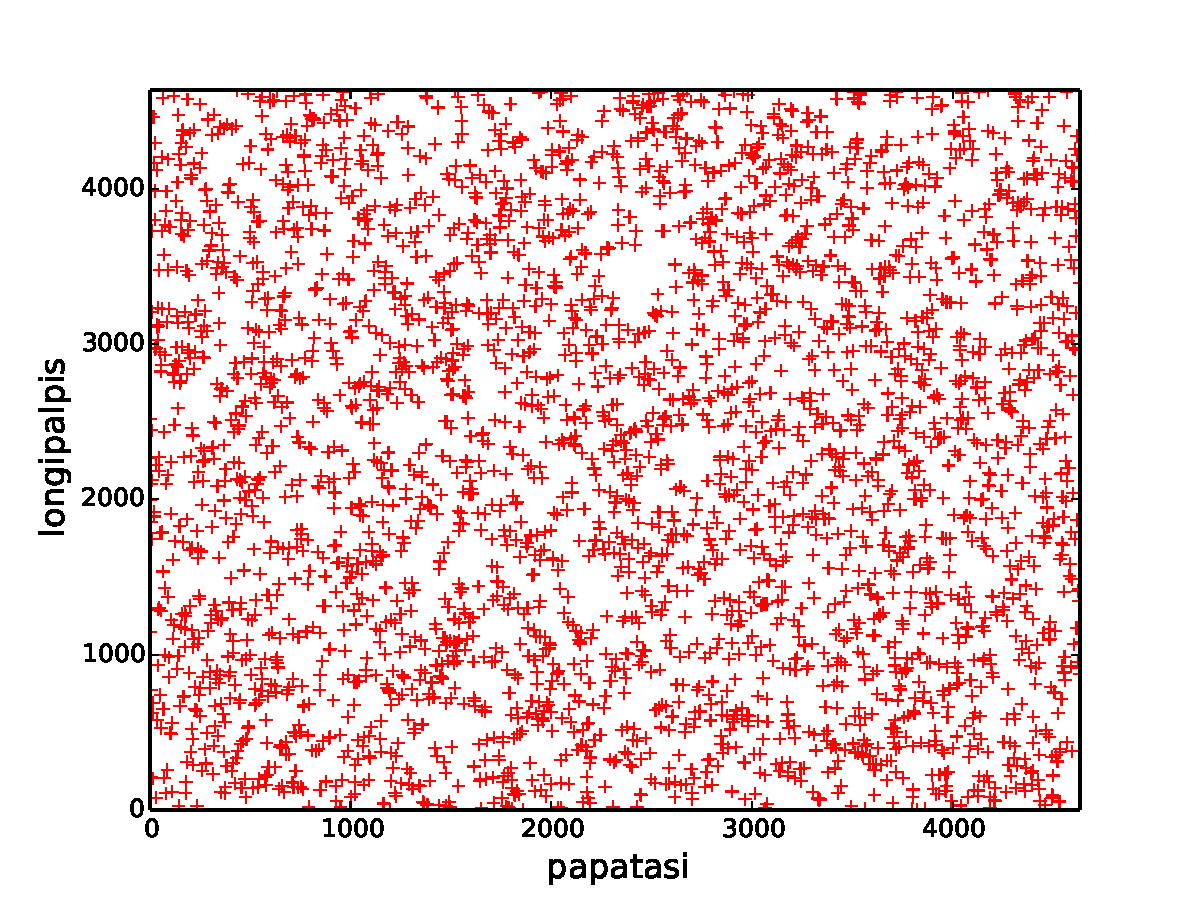
\includegraphics[width=\textwidth]{figures/synteny/papatasi_longipalpis_plot}
    \caption{\emph{L. longipalpis} vs. \emph{P. papatasi}}
  \end{subfigure}
  ~
  \begin{subfigure}[b]{0.45\textwidth}
    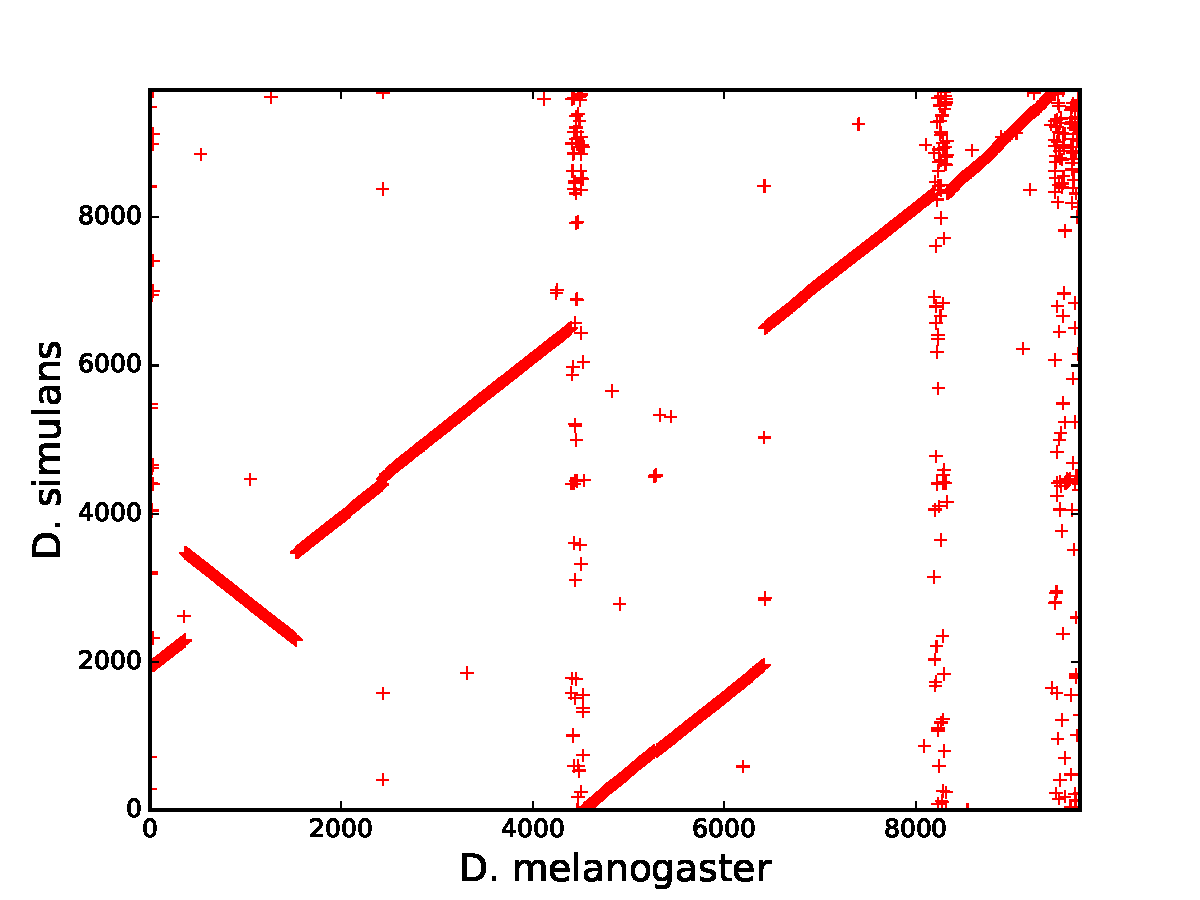
\includegraphics[width=\textwidth]{figures/synteny/dmel_dsim_plot}
    \caption{\emph{D. melanogaster} vs. \emph{D. simulans}}
  \end{subfigure}
  ~
  \begin{subfigure}[b]{0.45\textwidth}
    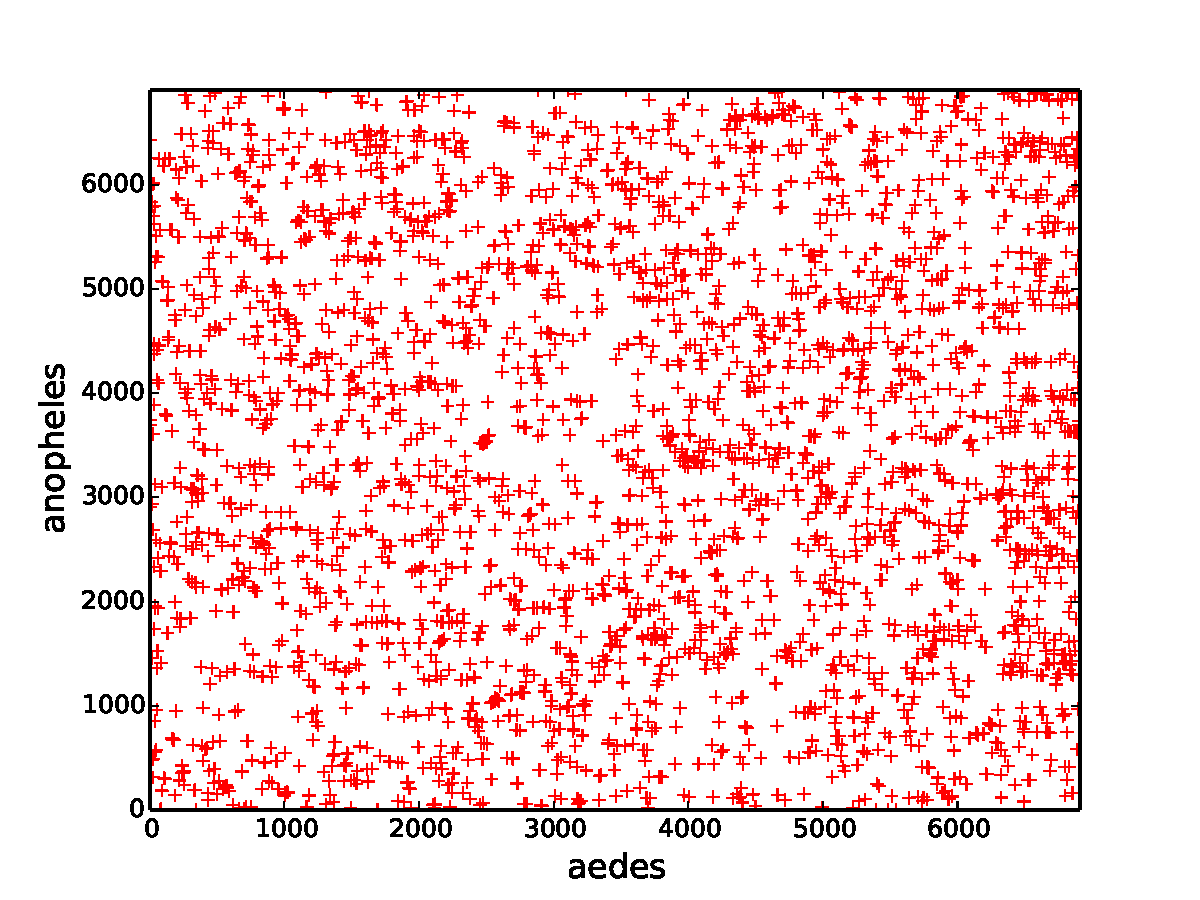
\includegraphics[width=\textwidth]{figures/synteny/aedes_anopheles_plot}
    \caption{\emph{Ae. aegypti} vs. \emph{A. gambiae}}
  \end{subfigure}
  ~
  \begin{subfigure}[b]{0.45\textwidth}
    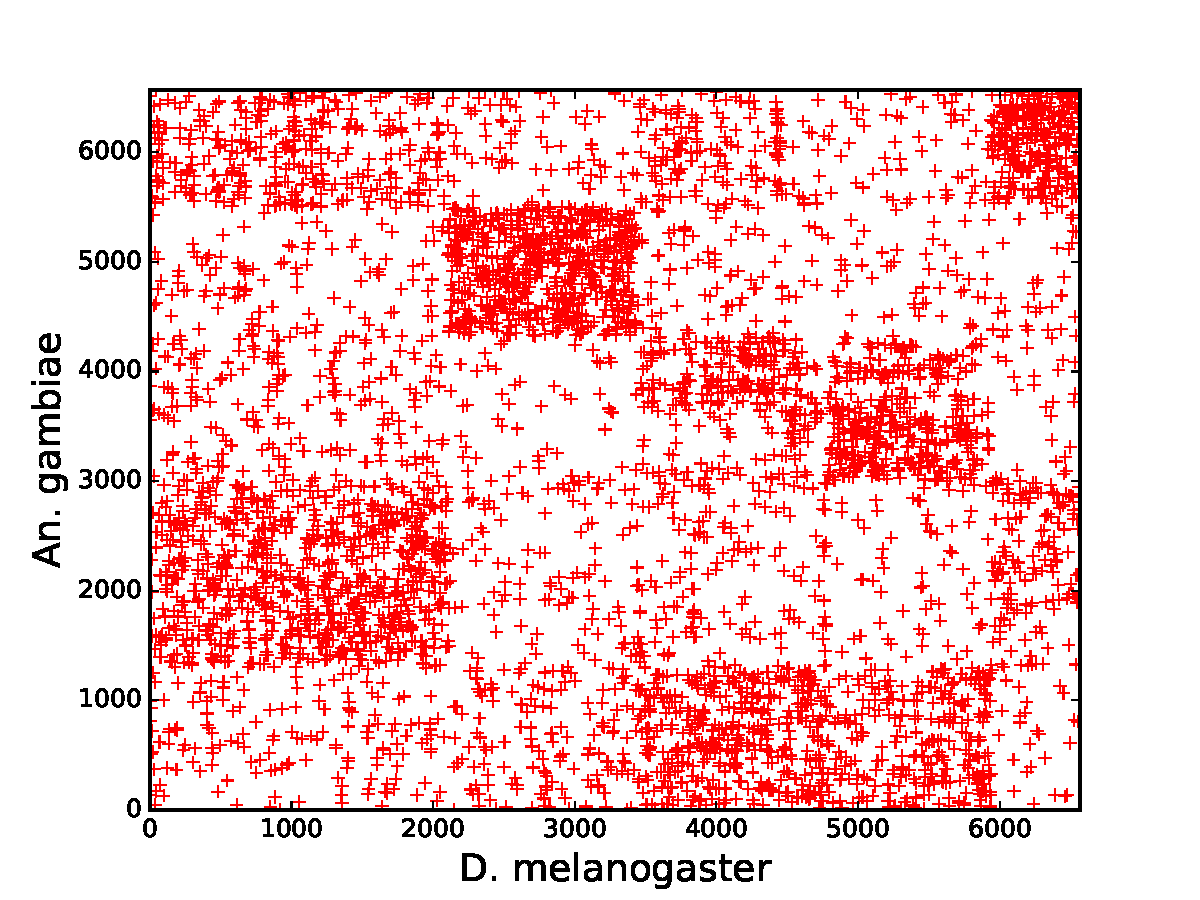
\includegraphics[width=\textwidth]{figures/synteny/dmel_anopheles_plot}
    \caption{\emph{A. gambiae} vs. \emph{D. melanogaster}}
  \end{subfigure}
\label{fig:dot-plots}
\end{figure}

\subsubsection{Microsynteny}

\textcolor{red}{block size distributions}

\textcolor{red}{analysis of individual blocks}

\subsection{Discussion and Conclusion}